% ============================================================
%  يُترجَم بـ XeLaTeX  (في Overleaf: Menu → Compiler → XeLaTeX)
%  الخط: Amiri (متوفر في Overleaf، أو حمّله من github.com/aliftype/amiri)
% ============================================================
\documentclass[12pt,a4paper]{article}
\usepackage[a4paper,margin=1.7cm,top=2.3cm,bottom=2.9cm,headheight=15pt,footskip=1.5cm]{geometry}
\usepackage{amsmath,amssymb}
\usepackage{icomma}
\usepackage[english,bidi=default,layout=lists]{babel}
\babelprovide[import,main]{arabic}
\babelfont{rm}[Scale=1.08]{Amiri}
\babelfont{sf}[Scale=1.08]{Amiri}
\usepackage[most]{tcolorbox}
\usepackage{tikz}
\usetikzlibrary{arrows.meta,calc,shadings}
\usepackage{array}
\usepackage{colortbl}
\usepackage{fancyhdr}
\usepackage{titlesec}
\usepackage{enumitem}
\usepackage{collcell}
\usepackage{needspace}
\usepackage{etoolbox}
% أعمدة جداول تُكتب خلاياها بالعربية في الاتجاه الصحيح
\newcolumntype{C}{>{\collectcell\ar}c<{\endcollectcell}}
% تجنب عنوان يتيم في أسفل الصفحة
\pretocmd{\section}{\Needspace{15\baselineskip}}{}{}
\pretocmd{\subsection}{\Needspace{11\baselineskip}}{}{}

% ---------- الألوان ----------
\definecolor{cDef}{HTML}{1F4E9C}
\definecolor{cThm}{HTML}{B3261E}
\definecolor{cRem}{HTML}{2E7D32}
\definecolor{cEx}{HTML}{C76B00}
\definecolor{cMeth}{HTML}{6A1B9A}
\definecolor{cSol}{HTML}{00695C}
\definecolor{cSec}{HTML}{1F3A68}

% ---------- العناوين ----------
\titleformat{\section}{\Large\bfseries\color{cSec}}{\thesection.}{0.6em}{}[{\color{cSec!60}\titlerule[1pt]}]
\titleformat{\subsection}{\large\bfseries\color{cThm!85!black}}{\thesubsection.}{0.5em}{}
\titlespacing*{\section}{0pt}{14pt}{8pt}
\titlespacing*{\subsection}{0pt}{10pt}{5pt}
\setlength{\parindent}{0pt}
\setlength{\parskip}{4pt}
\setlist{itemsep=2pt,topsep=3pt}

% ---------- الصناديق (تُرسم في سياق LTR ويُكتب محتواها بالعربية) ----------
\newtcolorbox{arbox}[3][]{enhanced,
  colback=#2!5,colframe=#2!80!black,arc=2mm,boxrule=0.8pt,
  left=6pt,right=6pt,top=8pt,bottom=5pt,
  fonttitle=\bfseries,coltitle=white,
  title={\foreignlanguage{arabic}{#3}},
  attach boxed title to top right={xshift=-5mm,yshift=-3mm},
  boxed title style={colback=#2!80!black,arc=1.5mm,boxrule=0pt},
  before upper={\selectlanguage{arabic}},
  before skip=8pt,after skip=8pt,#1}
\newenvironment{BOX}[2]{\begin{otherlanguage}{english}\begin{arbox}{#1}{#2}}{\end{arbox}\end{otherlanguage}}
\newenvironment{tarif}[1][تعريف]{\begin{BOX}{cDef}{#1}}{\end{BOX}}
\newenvironment{khassia}[1][خاصية]{\begin{BOX}{cThm}{#1}}{\end{BOX}}
\newenvironment{molahada}[1][ملاحظة]{\begin{BOX}{cRem}{#1}}{\end{BOX}}
\newenvironment{mithal}[1][مثال]{\begin{BOX}{cEx}{#1}}{\end{BOX}}
\newenvironment{tariqa}[1][طريقة]{\begin{BOX}{cMeth}{#1}}{\end{BOX}}

% ---------- التمارين والحلول ----------
\newcounter{exo}
\newenvironment{tamrin}[1]{\stepcounter{exo}\begin{BOX}{cSec}{التمرين \theexo: #1}}{\end{BOX}}
\newenvironment{hal}{\Needspace{12\baselineskip}\begin{otherlanguage}{english}\begin{arbox}[breakable]{cSol}{حل التمرين \theexo}}{\end{arbox}\end{otherlanguage}}

% رسومات TikZ تُوضع في سياق LTR
\newenvironment{LTR}{\begin{otherlanguage}{english}}{\end{otherlanguage}}
\newcommand{\ar}[1]{\foreignlanguage{arabic}{#1}}

% ---------- رموز ----------
% نقاط الحذف داخل الرياضيات (\dots يسبب خللاً في الاتجاه مع babel)
\renewcommand{\dots}{\mathinner{\ldotp\ldotp\ldotp}}
\renewcommand{\ldots}{\mathinner{\ldotp\ldotp\ldotp}}
\renewcommand{\cdots}{\mathinner{\cdotp\cdotp\cdotp}}
\newcommand{\N}{\mathbb{N}}
\newcommand{\Z}{\mathbb{Z}}
\newcommand{\D}{\mathbb{D}}
\newcommand{\Q}{\mathbb{Q}}
\newcommand{\R}{\mathbb{R}}
\newcommand{\pgcd}{\operatorname{PGCD}}
\newcommand{\ppcm}{\operatorname{PPCM}}

% ---------- تمثيل مجال على مستقيم عددي ----------
% \NLseg{a}{b}{[}{]}  مجال محدود
\newcommand{\NLseg}[4]{\begin{LTR}\begin{tikzpicture}[baseline=-0.6ex]
 \draw[-{Stealth[length=2mm]},gray!70](0,0)--(3.4,0);
 \draw[line width=2pt,cThm!80!black](0.7,0)--(2.7,0);
 \node[cThm!80!black,font=\LARGE] at (0.7,0){$#3$};
 \node[cThm!80!black,font=\LARGE] at (2.7,0){$#4$};
 \node[below=3pt,font=\footnotesize] at (0.7,0){$#1$};
 \node[below=3pt,font=\footnotesize] at (2.7,0){$#2$};
\end{tikzpicture}\end{LTR}}
% \NLright{a}{[}  مجال نحو +∞
\newcommand{\NLright}[2]{\begin{LTR}\begin{tikzpicture}[baseline=-0.6ex]
 \draw[-{Stealth[length=2mm]},gray!70](0,0)--(3.4,0);
 \draw[line width=2pt,cThm!80!black](1.3,0)--(3.3,0);
 \node[cThm!80!black,font=\LARGE] at (1.3,0){$#2$};
 \node[below=3pt,font=\footnotesize] at (1.3,0){$#1$};
\end{tikzpicture}\end{LTR}}
% \NLleft{b}{]}  مجال نحو −∞
\newcommand{\NLleft}[2]{\begin{LTR}\begin{tikzpicture}[baseline=-0.6ex]
 \draw[-{Stealth[length=2mm]},gray!70](0,0)--(3.4,0);
 \draw[line width=2pt,cThm!80!black](0.05,0)--(2.1,0);
 \node[cThm!80!black,font=\LARGE] at (2.1,0){$#2$};
 \node[below=3pt,font=\footnotesize] at (2.1,0){$#1$};
\end{tikzpicture}\end{LTR}}

% ---------- أيقونات مواقع التواصل (مرسومة بـ TikZ، لا تحتاج أي حزمة) ----------
\definecolor{cFB}{HTML}{1877F2}
\definecolor{cTG}{HTML}{229ED9}
\definecolor{cIG1}{HTML}{FEDA75}
\definecolor{cIG2}{HTML}{D62976}
\definecolor{cIG3}{HTML}{4F5BD5}
\newcommand{\fbicon}{\begin{LTR}\begin{tikzpicture}[baseline=-0.75ex,x=1em,y=1em]
 \fill[cFB] (0,0) circle (0.55);
 \node[white,inner sep=0,font=\usefont{TU}{lmss}{bx}{n}\small] at (0.04,-0.02) {f};
\end{tikzpicture}\end{LTR}}
\newcommand{\igicon}{\begin{LTR}
\begin{tikzpicture}[baseline=-0.75ex,x=1em,y=1em]
 \shade[lower left=cIG1,lower right=cIG2,upper left=cIG2,upper right=cIG3,rounded corners=0.28em] (-0.55,-0.55) rectangle (0.55,0.55);
 \draw[white,line width=0.09em,rounded corners=0.18em] (-0.36,-0.36) rectangle (0.36,0.36);
 \draw[white,line width=0.09em] (0,0) circle (0.17);
 \fill[white] (0.22,0.22) circle (0.05);
\end{tikzpicture}\end{LTR}}
\newcommand{\tgicon}{\begin{LTR}
\begin{tikzpicture}[baseline=-0.75ex,x=1em,y=1em]
 \fill[cTG] (0,0) circle (0.55);
 \fill[white] (-0.33,0.0) -- (0.32,0.27) -- (0.2,-0.3) -- (0.0,-0.15) -- (-0.08,-0.28) -- (-0.08,-0.08) -- cycle;
 \fill[cTG!70!black] (-0.08,-0.08) -- (0.25,0.2) -- (0.0,-0.15) -- (-0.08,-0.28) -- cycle;
\end{tikzpicture}\end{LTR}}
% سطر مواقع التواصل أسفل كل صفحة
% (يُكتب السطر بترتيب بصري من اليسار إلى اليمين: الأيقونة يمين كل اسم)
\newcommand{\SocialRow}{\begin{otherlanguage}{english}%
 \ar{\textbf{الأستاذ سوايسية هشام للرياضيات}}\ \tgicon\hfill
 \textbf{prof\_hicham\_math}\ \igicon\hfill
 \ar{\textbf{الأستاذ سوايسية هشام للرياضيات}}\ \fbicon\end{otherlanguage}}

% ---------- رأس وتذييل الصفحة ----------
\pagestyle{fancy}
\fancyhf{}
\renewcommand{\headrulewidth}{0.6pt}
\renewcommand{\footrulewidth}{0.4pt}
% \SetHeader{يمين الرأس}{يسار الرأس}{يمين التذييل}{يسار التذييل}
\newcommand{\SetHeader}[4]{%
 \fancyhead[C]{\parbox{\textwidth}{\ar{#1\hfill #2}}}%
 \fancyfoot[C]{\parbox{\textwidth}{\ar{#3\hfill #4}\\[3pt]
   \rule{\textwidth}{0.3pt}\\[1pt]
   \footnotesize\SocialRow}}}


% ---------- رسم بياني مصغر: \MiniG{العبارة}{بداية}{نهاية}{ymin}{ymax}
\newcommand{\MiniG}[5]{\begin{LTR}\begin{tikzpicture}[scale=0.42,baseline=(current bounding box.center)]
 \draw[gray!30,very thin] (-3,#4) grid (3,#5);
 \draw[-{Stealth[length=1.5mm]}] (-3.2,0)--(3.3,0);
 \draw[-{Stealth[length=1.5mm]}] (0,#4-0.2)--(0,#5+0.3);
 \draw[cThm,very thick,smooth,samples=60,domain=#2:#3] plot (\x,{#1});
\end{tikzpicture}\end{LTR}}

\SetHeader{\small\bfseries\color{cSec}الوحدة الأولى: الدوال العددية}{\small\color{cSec}السنة الثانية ثانوي -- الشعب العلمية}{\small الأستاذ سوايسية هشام}{\small ملخص الوحدة -- صفحة \thepage}

\begin{document}

\begin{LTR}
\begin{tcolorbox}[enhanced,colback=cSec,colframe=cSec,arc=3mm,halign=center,
  boxrule=0pt,top=10pt,bottom=10pt,before upper={\selectlanguage{arabic}}]
{\color{white}\Huge\bfseries ملخص الوحدة الأولى: الدوال العددية}\\[6pt]
{\color{white}\large السنة الثانية ثانوي -- علوم تجريبية، رياضيات، تقني رياضي}\\[4pt]
{\color{white!85!cSec}\normalsize إعداد: الأستاذ سوايسية هشام}
\end{tcolorbox}
\end{LTR}

\begin{BOX}{cSec}{محتوى الملخص}
\begin{enumerate}
\item تذكير بقواعد الحساب.
\item عموميات: مجموعة التعريف، اتجاه التغير، الدوال المرجعية.
\item العمليات على الدوال وتساوي دالتين.
\item تركيب دالتين وتفكيك دالة.
\item اتجاه تغير الدوال $f+k$ ، $\lambda f$ ، $g\circ f$.
\item التمثيلات البيانية المستنتجة من تمثيل بياني معلوم.
\item دساتير تغيير المعلم، الشفعية، محور ومركز التناظر.
\item التقاطع مع المحورين والمناقشة البيانية.
\item كثيرات الحدود وتحليلها: المطابقة ، القسمة الإقليدية وجدول هورنر.
\item المعادلات والمتراجحات من الدرجة الثانية ومضاعفة التربيع.
\end{enumerate}
\end{BOX}

% =================================================
\section{تذكير بقواعد الحساب}
% =================================================
\begin{khassia}[المتطابقات الشهيرة]
\begin{center}
\renewcommand{\arraystretch}{1.5}
\begin{tabular}{|C|C|}\hline
\textbf{من الدرجة الثالثة} & \textbf{من الدرجة الثانية}\\\hline
$(a+b)^3=a^3+3a^2b+3ab^2+b^3$ & $(a+b)^2=a^2+2ab+b^2$\\
$(a-b)^3=a^3-3a^2b+3ab^2-b^3$ & $(a-b)^2=a^2-2ab+b^2$\\
$a^3-b^3=(a-b)\left(a^2+ab+b^2\right)$ & $a^2-b^2=(a-b)(a+b)$\\
 $a^3+b^3=(a+b)\left(a^2-ab+b^2\right)$ & \\\hline
\end{tabular}
\end{center}
\end{khassia}
\begin{khassia}[القيمة المطلقة]
\[|x|=\begin{cases}x & x\ge0\\-x & x\le0\end{cases}\qquad \sqrt{x^2}=|x|\qquad |xy|=|x|\,|y|\qquad |x+y|\le|x|+|y|\]
\[|x|\le a\iff-a\le x\le a\qquad;\qquad |x|\ge a\iff x\le-a\ \ \text{أو}\ \ x\ge a\qquad(a>0)\]
\end{khassia}

% =================================================
\section{عموميات حول الدوال}
% =================================================
\begin{tarif}[الدالة ومجموعة التعريف]
\begin{itemize}
\item الدالة $f$ تُرفق بكل عدد حقيقي $x$ من مجموعة $D_f$ عدداً حقيقياً وحيداً $f(x)$ يسمى \textbf{صورة} $x$.
\item $D_f$ مجموعة الأعداد الحقيقية $x$ التي يكون من أجلها حساب $f(x)$ ممكناً.
\item إذا كان $f(x)=\beta$ فإن $x$ \textbf{سابقة} للعدد $\beta$ ؛ ولتعيين السوابق نحل المعادلة $f(x)=\beta$.
\end{itemize}
\end{tarif}
\begin{tariqa}[تعيين مجموعة التعريف]
\begin{center}
\renewcommand{\arraystretch}{1.6}
\begin{tabular}{|C|C|}\hline
\textbf{الشرط} & \textbf{شكل الدالة}\\\hline
$D_f=\R$ & كثير حدود\\\hline
$v(x)\neq0$ & $f(x)=\dfrac{u(x)}{v(x)}$\\\hline
$u(x)\ge0$ & $f(x)=\sqrt{u(x)}$\\\hline
$u(x)>0$ & $f(x)=\dfrac{1}{\sqrt{u(x)}}$\\\hline
\end{tabular}
\end{center}
في حالة مجموع أو فرق أو جداء أو قسمة دالتين أو أكثر، تكون $D_f$ تقاطع مجموعات تعريف هذه الدوال.
\end{tariqa}
\begin{tarif}[التمثيل البياني]
التمثيل البياني $(C_f)$ للدالة $f$ في معلم $\left(O;\vec i,\vec j\right)$ هو مجموعة النقط $M(x;y)$ حيث $x\in D_f$ و $y=f(x)$.
نقول إن $y=f(x)$ معادلة للمنحنى $(C_f)$.
\end{tarif}
\begin{tarif}[اتجاه التغير على مجال $I$]
من أجل كل عددين $x_1$ و $x_2$ من $I$ حيث $x_1<x_2$:
\begin{itemize}
\item $f$ \textbf{متزايدة تماماً} على $I$ إذا كان $f(x_1)<f(x_2)$ (تحافظ على الترتيب).
\item $f$ \textbf{متناقصة تماماً} على $I$ إذا كان $f(x_1)>f(x_2)$ (تعكس الترتيب).
\item $f$ \textbf{ثابتة} على $I$ إذا كان $f(x_1)=f(x_2)$.
\end{itemize}
نقول إن $f$ \textbf{رتيبة} على $I$ إذا كانت متزايدة أو متناقصة على $I$.\\
\textbf{تنبيه:} لا علاقة بين اتجاه تغير دالة وإشارتها.
\end{tarif}
\begin{khassia}[صورة مجال بدالة رتيبة تماماً]
إذا كانت $f$ متزايدة تماماً على $[a;b]$ فإن $f\big([a;b]\big)=\big[f(a);f(b)\big]$ ،
وإذا كانت متناقصة تماماً فإن $f\big([a;b]\big)=\big[f(b);f(a)\big]$.
\end{khassia}

\subsection{الدوال المرجعية}
\begin{khassia}[الدوال المرجعية]
\begin{center}
\renewcommand{\arraystretch}{1.25}
\begin{tabular}{|>{\centering\arraybackslash}m{3.6cm}|>{\centering\arraybackslash}m{7cm}|>{\centering\arraybackslash}m{2.8cm}|}\hline
\textbf{التمثيل البياني} & \textbf{اتجاه التغير} & \textbf{الدالة}\\\hline
\MiniG{\x*\x}{-1.9}{1.9}{-0.5}{3.6} & متناقصة تماماً على $]-\infty;0]$ ومتزايدة تماماً على $[0;+\infty[$ & مربع\newline $x\mapsto x^2$\\\hline
\begin{LTR}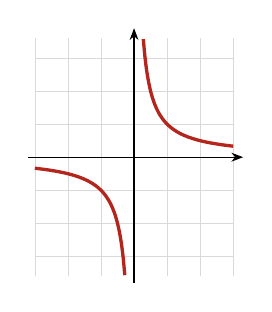
\begin{tikzpicture}[scale=0.42,baseline=(current bounding box.center)]
 \draw[gray!30,very thin] (-3,-3.6) grid (3,3.6);
 \draw[-{Stealth[length=1.5mm]}] (-3.2,0)--(3.3,0);
 \draw[-{Stealth[length=1.5mm]}] (0,-3.8)--(0,3.9);
 \draw[cThm,very thick,smooth,samples=60,domain=0.28:3] plot (\x,{1/\x});
 \draw[cThm,very thick,smooth,samples=60,domain=-3:-0.28] plot (\x,{1/\x});
\end{tikzpicture}\end{LTR} & متناقصة تماماً على $]-\infty;0[$ وعلى $]0;+\infty[$ & مقلوب\newline $x\mapsto\dfrac1x$\\\hline
\MiniG{sqrt(\x)}{0}{3}{-0.5}{2} & متزايدة تماماً على $[0;+\infty[$ & الجذر التربيعي\newline $x\mapsto\sqrt x$\\\hline
\MiniG{abs(\x)}{-2.8}{2.8}{-0.5}{3} & متناقصة تماماً على $]-\infty;0]$ ومتزايدة تماماً على $[0;+\infty[$ & القيمة المطلقة\newline $x\mapsto|x|$\\\hline
\MiniG{\x*\x*\x}{-1.5}{1.5}{-3.4}{3.4} & متزايدة تماماً على $\R$ & مكعب\newline $x\mapsto x^3$\\\hline
\end{tabular}
\end{center}
\end{khassia}

% =================================================
\section{العمليات على الدوال}
% =================================================
\begin{tarif}[تساوي دالتين]
القول عن دالتين $f$ و $g$ إنهما متساويتان يعني أن لهما \textbf{نفس مجموعة التعريف} $D$ ، وأنه من أجل كل $x$ من $D$: $f(x)=g(x)$. ونكتب $f=g$.
\end{tarif}
\begin{mithal}
$f(x)=\dfrac{x^2+3x+2}{x+2}$ و $g(x)=x+1$: \quad $D_f=\R-\{-2\}$ و $D_g=\R$.\\
من أجل $x\neq-2$: $f(x)=\dfrac{(x+2)(x+1)}{x+2}=x+1=g(x)$ ، لكن $D_f\neq D_g$ إذن $f\neq g$.
\end{mithal}
\begin{tarif}[العمليات الجبرية ($k$ و $\lambda$ عددان حقيقيان)]
\begin{center}
\renewcommand{\arraystretch}{1.65}
\begin{tabular}{|C|C|C|C|}\hline
\textbf{مجموعة التعريف} & \textbf{التعريف} & \textbf{الرمز} & \textbf{العملية}\\\hline
$D_f$ & $(f+k)(x)=f(x)+k$ & $f+k$ & مجموع $f$ و $k$\\\hline
$D_f\cap D_g$ & $(f+g)(x)=f(x)+g(x)$ & $f+g$ & مجموع $f$ و $g$\\\hline
$D_f$ & $(\lambda f)(x)=\lambda f(x)$ & $\lambda f$ & جداء $f$ بالعدد $\lambda$\\\hline
$D_f\cap D_g$ & $(f\times g)(x)=f(x)\times g(x)$ & $f\times g$ & جداء $f$ و $g$\\\hline
$D_f\cap D_g$ \ و \ $g(x)\neq0$ & $\left(\dfrac fg\right)(x)=\dfrac{f(x)}{g(x)}$ & $\dfrac fg$ & حاصل قسمة $f$ على $g$\\\hline
\end{tabular}
\end{center}
\end{tarif}

% =================================================
\section{تركيب دالتين وتفكيك دالة}
% =================================================
\begin{tarif}[مركب دالتين]
$f$ و $g$ دالتان معرفتان على $D_f$ و $D_g$. مركب الدالة $f$ متبوعة بالدالة $g$ هي الدالة $g\circ f$ المعرفة بـ:
\[(g\circ f)(x)=g\big(f(x)\big)\qquad\text{حيث}\qquad D_{g\circ f}=\big\{x\in D_f\ :\ f(x)\in D_g\big\}\]
\end{tarif}
\begin{mithal}
$f(x)=x-3$ و $g(x)=\sqrt x$:
\begin{itemize}
\item $g\circ f$: $x\in\R$ و $x-3\ge0$ ، إذن $D_{g\circ f}=[3;+\infty[$ و $(g\circ f)(x)=\sqrt{x-3}$.
\item $f\circ g$: $x\ge0$ ، إذن $D_{f\circ g}=[0;+\infty[$ و $(f\circ g)(x)=\sqrt x-3$.
\end{itemize}
\textbf{نلاحظ:} $g\circ f\neq f\circ g$ ؛ تركيب الدوال ليس تبديلياً.
\end{mithal}
\begin{tariqa}[تفكيك دالة إلى مركب دالتين مرجعيتين]
\begin{center}
\renewcommand{\arraystretch}{1.6}
\begin{tabular}{|C|C|C|}\hline
\textbf{الدالة الخارجية} $v$ & \textbf{الدالة الداخلية} $u$ & \textbf{شكل الدالة}\\\hline
$v(x)=x^2+b$ & $u(x)$ & $f(x)=\big[u(x)\big]^2+b$\\\hline
$v(x)=\sqrt x+b$ & $u(x)$ & $f(x)=\sqrt{u(x)}+b$\\\hline
$v(x)=\dfrac1x+b$ & $u(x)$ & $f(x)=\dfrac{1}{u(x)}+b$\\\hline
$v(x)=|x|$ & $u(x)$ & $f(x)=\big|u(x)\big|$\\\hline
\end{tabular}
\end{center}
وفي كل حالة: $f=v\circ u$. \quad مثال: $f(x)=2x^2+1=v\big(u(x)\big)$ حيث $u(x)=x^2$ و $v(x)=2x+1$.
\end{tariqa}

% =================================================
\section{اتجاه تغير الدوال $f+k$ ، $\lambda f$ ، $g\circ f$}
% =================================================
\begin{khassia}[مبرهنات]
$f$ دالة رتيبة تماماً على مجال $I$ ، و $k$ و $\lambda$ عددان حقيقيان ($\lambda\ne0$).
\begin{center}
\renewcommand{\arraystretch}{1.5}
\begin{tabular}{|>{\centering\arraybackslash}m{12.6cm}|>{\centering\arraybackslash}m{2.4cm}|}\hline
\textbf{اتجاه التغير} & \textbf{الدالة}\\\hline
للدالتين $f$ و $f+k$ نفس اتجاه التغير على $I$. & $f+k$\\\hline
إذا كان $\lambda>0$: لـ $f$ و $\lambda f$ نفس اتجاه التغير ؛ وإذا كان $\lambda<0$: اتجاها تغيرهما متعاكسان. & $\lambda f$\\\hline
($g$ رتيبة تماماً على مجال $J$ يشمل $f(I)$) \newline إذا كان لـ $f$ و $g$ نفس اتجاه التغير فإن $g\circ f$ \textbf{متزايدة تماماً} على $I$ ؛\newline وإذا كان اتجاها تغيرهما متعاكسين فإن $g\circ f$ \textbf{متناقصة تماماً} على $I$. & $g\circ f$\\\hline
\end{tabular}
\end{center}
\end{khassia}
\begin{molahada}
\begin{itemize}
\item مجموع دالتين متزايدتين تماماً على $I$ هو دالة متزايدة تماماً على $I$ (وكذلك للمتناقصتين).
\item لا يمكن إعطاء قاعدة عامة لاتجاه تغير $f+g$ و $f\times g$ في كل الحالات.
\end{itemize}
\end{molahada}
\begin{mithal}
\begin{itemize}
\item $f(x)=2\sqrt x+3$: الدالة $x\mapsto\sqrt x$ متزايدة تماماً على $[0;+\infty[$ و $2>0$ ، إذن $f$ متزايدة تماماً على $[0;+\infty[$.
\item $g(x)=\sqrt{-x+2}$ على $]-\infty;2]$: $u(x)=-x+2$ متناقصة و $v(x)=\sqrt x$ متزايدة، إذن $g=v\circ u$ متناقصة تماماً.
\end{itemize}
\end{mithal}

% =================================================
\section{التمثيلات البيانية المستنتجة}
% =================================================
\begin{khassia}[استنتاج $(C_g)$ انطلاقاً من $(C_f)$ \ ($a$ ، $b$ ، $\lambda$ أعداد حقيقية)]
\begin{center}
\renewcommand{\arraystretch}{1.45}
\begin{tabular}{|>{\centering\arraybackslash}m{9.4cm}|>{\centering\arraybackslash}m{2.6cm}|>{\centering\arraybackslash}m{3.2cm}|}\hline
\textbf{التحويل} & \textbf{شرط الوجود} & \textbf{عبارة} $g(x)$\\\hline
$(C_g)$ صورة $(C_f)$ بالانسحاب الذي شعاعه $b\,\vec j$ & $x\in D_f$ & $f(x)+b$\\\hline
$(C_g)$ صورة $(C_f)$ بالانسحاب الذي شعاعه $-a\,\vec i$ & $x+a\in D_f$ & $f(x+a)$\\\hline
$(C_g)$ صورة $(C_f)$ بالانسحاب الذي شعاعه $\vec v\binom{-a}{b}$ & $x+a\in D_f$ & $f(x+a)+b$\\\hline
نضرب ترتيب كل نقطة من $(C_f)$ في $\lambda$ & $x\in D_f$ & $\lambda f(x)$\\\hline
$(C_g)$ نظير $(C_f)$ بالنسبة لمحور الفواصل & $x\in D_f$ & $-f(x)$\\\hline
$(C_g)$ نظير $(C_f)$ بالنسبة لمحور التراتيب & $-x\in D_f$ & $f(-x)$\\\hline
$(C_g)$ نظير $(C_f)$ بالنسبة لمبدأ المعلم & $-x\in D_f$ & $-f(-x)$\\\hline
ينطبق على $(C_f)$ حيث $f(x)\ge0$ ، ويناظره بالنسبة لمحور الفواصل حيث $f(x)<0$ & $x\in D_f$ & $\big|f(x)\big|$\\\hline
$g$ زوجية: ينطبق على $(C_f)$ من أجل $x\ge0$ ، ثم نكمل بالتناظر بالنسبة لمحور التراتيب & $|x|\in D_f$ & $f\big(|x|\big)$\\\hline
\end{tabular}
\end{center}
\end{khassia}
\begin{mithal}[مثال: $f(x)=x^2-3$ و $g(x)=|f(x)|$]
\begin{minipage}{0.52\textwidth}
\begin{itemize}
\item $(C_f)$ صورة منحنى الدالة مربع بالانسحاب الذي شعاعه $-3\vec j$.
\item $(C_g)$ ينطبق على $(C_f)$ لما $f(x)\ge0$ ، أي لما $x\le-\sqrt3$ أو $x\ge\sqrt3$.
\item لما $-\sqrt3<x<\sqrt3$ يكون $(C_g)$ نظير $(C_f)$ بالنسبة لمحور الفواصل.
\end{itemize}
\end{minipage}\hfill
\begin{minipage}{0.44\textwidth}
\centering
\begin{LTR}
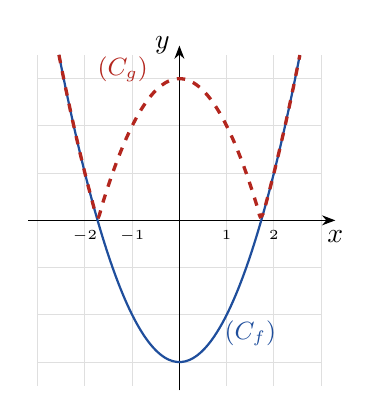
\begin{tikzpicture}[scale=0.6]
 \draw[gray!25] (-3,-3.5) grid (3,3.5);
 \draw[-{Stealth}] (-3.2,0)--(3.3,0) node[below]{$x$};
 \draw[-{Stealth}] (0,-3.6)--(0,3.7) node[left]{$y$};
 \foreach \t in {-2,-1,1,2} \node[below,font=\tiny] at (\t,0){$\t$};
 \draw[cDef,thick,smooth,samples=60,domain=-2.55:2.55] plot (\x,{\x*\x-3});
 \draw[cThm,very thick,dashed,smooth,samples=80,domain=-2.55:2.55] plot (\x,{abs(\x*\x-3)});
 \node[cDef,font=\small] at (1.5,-2.4){$(C_f)$};
 \node[cThm,font=\small] at (-1.2,3.2){$(C_g)$};
\end{tikzpicture}
\end{LTR}
\end{minipage}
\end{mithal}

% =================================================
\section{تغيير المعلم، الشفعية والتناظر}
% =================================================
\begin{khassia}[دساتير تغيير المعلم]
$\Omega(x_0;y_0)$ نقطة من المستوي. إذا كانت $(x;y)$ إحداثيي نقطة $M$ في المعلم $\left(O;\vec i,\vec j\right)$ و $(X;Y)$ إحداثييها في المعلم $\left(\Omega;\vec i,\vec j\right)$ فإن:
\[\begin{cases}x=X+x_0\\ y=Y+y_0\end{cases}\]
وتُستنتج هذه الدساتير من علاقة شال: \ $\overrightarrow{OM}=\overrightarrow{O\Omega}+\overrightarrow{\Omega M}$.
\end{khassia}
\begin{tarif}[الشفعية]
\begin{center}
\renewcommand{\arraystretch}{1.5}
\begin{tabular}{|>{\centering\arraybackslash}m{5.8cm}|>{\centering\arraybackslash}m{6.8cm}|>{\centering\arraybackslash}m{2.6cm}|}\hline
 \textbf{التفسير الهندسي} & \textbf{التعريف} & \\\hline
$(C_f)$ متناظر بالنسبة لمحور التراتيب & $D_f$ متناظرة بالنسبة لـ $0$ و $f(-x)=f(x)$ & دالة زوجية\\\hline
$(C_f)$ متناظر بالنسبة لمبدأ المعلم & $D_f$ متناظرة بالنسبة لـ $0$ و $f(-x)=-f(x)$ & دالة فردية\\\hline
$(C_f)$ يعيد نفسه على كل مجال طوله $T$ & $f(x+T)=f(x)$ & دالة دورية\\\hline
\end{tabular}
\end{center}
\end{tarif}
\begin{khassia}[محور التناظر ومركز التناظر]
\begin{center}
\renewcommand{\arraystretch}{1.5}
\begin{tabular}{|>{\centering\arraybackslash}m{7.5cm}|>{\centering\arraybackslash}m{7.5cm}|}\hline
\textbf{النقطة $\Omega(\alpha;\beta)$ مركز تناظر لـ $(C_f)$} & \textbf{المستقيم $x=\alpha$ محور تناظر لـ $(C_f)$}\\\hline
من أجل كل $x$ حيث $2\alpha-x\in D_f$: \newline $f(2\alpha-x)+f(x)=2\beta$ & من أجل كل $x$ حيث $2\alpha-x\in D_f$: \newline $f(2\alpha-x)=f(x)$\\\hline
أو: \ $f(\alpha-x)+f(\alpha+x)=2\beta$ & أو: \ $f(\alpha-x)=f(\alpha+x)$\\\hline
أو: في المعلم $(\Omega;\vec i,\vec j)$ ، الدالة $Y=f(\alpha+X)-\beta$ فردية & أو: في المعلم $(\Omega;\vec i,\vec j)$ حيث $\Omega(\alpha;0)$ ، الدالة $Y=f(\alpha+X)$ زوجية\\\hline
\end{tabular}
\end{center}
\end{khassia}
\begin{mithal}
\begin{itemize}
\item $f(x)=x^2+2x+1$: \ $f(-1+x)=x^2=f(-1-x)$ ، إذن المستقيم $x=-1$ محور تناظر لـ $(C_f)$.
\item $f(x)=\dfrac{3x-5}{x-2}$: نضع $x=X+2$ و $y=Y+3$ فنجد $Y+3=\dfrac{3X+1}{X}=3+\dfrac1X$ أي $Y=\dfrac1X$ ،
وهي دالة فردية، إذن $\Omega(2;3)$ مركز تناظر لـ $(C_f)$.
\end{itemize}
\end{mithal}

% =================================================
\section{التقاطع مع المحورين والمناقشة البيانية}
% =================================================
\begin{tariqa}[قراءات بيانية]
\begin{center}
\renewcommand{\arraystretch}{1.5}
\begin{tabular}{|>{\centering\arraybackslash}m{10.2cm}|>{\centering\arraybackslash}m{5cm}|}\hline
\textbf{كيفية الإجابة} & \textbf{السؤال}\\\hline
نحل المعادلة $f(x)=0$ & تقاطع $(C_f)$ مع محور الفواصل\\\hline
نحسب $f(0)$ (إذا كان $0\in D_f$) & تقاطع $(C_f)$ مع محور التراتيب\\\hline
فواصل النقط المشتركة بين $(C_f)$ و $(C_g)$ & حل المعادلة $f(x)=g(x)$ بيانياً\\\hline
فواصل نقط $(C_f)$ الواقعة فوق $(C_g)$ & حل المتراجحة $f(x)>g(x)$ بيانياً\\\hline
$f(x)>0$ حيث $(C_f)$ فوق محور الفواصل، و $f(x)<0$ حيث هو تحته & إشارة $f(x)$\\\hline
\end{tabular}
\end{center}
\end{tariqa}
\begin{tariqa}[المناقشة البيانية حسب قيم الوسيط $m$]
\begin{itemize}
\item حلول المعادلة $f(x)=m$ هي فواصل نقط تقاطع $(C_f)$ مع المستقيم الأفقي $y=m$ ؛ نحرك المستقيم ونعد نقط التقاطع.
\item حلول المعادلة $f(x)=x+m$ هي فواصل نقط تقاطع $(C_f)$ مع المستقيمات الموازية للمستقيم $y=x$.
\item حلول المعادلة $f(x)=mx+b$: مستقيمات دورانية تشمل النقطة الثابتة $A(0;b)$.
\end{itemize}
\end{tariqa}

% =================================================
\section{كثيرات الحدود}
% =================================================
\subsection{تعاريف}
\begin{tarif}[كثير حدود ، درجته ومعاملاته]
\begin{itemize}
\item نسمي \textbf{كثير حدود} كل دالة $f$ معرفة على $\R$ بـ: $f(x)=a_nx^n+a_{n-1}x^{n-1}+\cdots+a_1x+a_0$ ، حيث $a_n,\ \ldots,\ a_1,\ a_0$ أعداد حقيقية تسمى \textbf{معاملاته}.
\item إذا كان $a_n\neq0$ فإن $n$ \textbf{درجة} كثير الحدود (أكبر أس للمتغير $x$ معامله غير معدوم) ، و $a_n$ \textbf{المعامل الرئيسي} ، و $a_0$ \textbf{الحد الثابت}.
\item كثير الحدود الذي كل معاملاته معدومة يسمى \textbf{كثير الحدود المعدوم} (ليست له درجة) ، والدالة الثابتة غير المعدومة كثير حدود من الدرجة $0$.
\item العدد الحقيقي $\alpha$ \textbf{جذر} لكثير الحدود $f$ إذا كان $f(\alpha)=0$.
\end{itemize}
\end{tarif}
\begin{mithal}
\begin{itemize}
\item $f(x)=2x^3-3x^2-11x+6$: الدرجة $3$ ، المعاملات بالترتيب: $2$ ، $-3$ ، $-11$ ، $6$ ؛ المعامل الرئيسي $2$ والحد الثابت $6$.
\item $h(x)=5x^4-x+1$: الدرجة $4$ ، ومعاملاته $5$ ، $0$ ، $0$ ، $-1$ ، $1$ (نكتب $0$ لكل أس غائب: $5x^4+0x^3+0x^2-x+1$).
\item $f(3)=54-27-33+6=0$ ، إذن العدد $3$ جذر لـ $f$ ؛ و $f(1)=2-3-11+6=-6\neq0$ ، إذن $1$ ليس جذراً.
\end{itemize}
\end{mithal}
\begin{khassia}[مبرهنات (مبدأ المطابقة)]
\begin{enumerate}
\item يكون كثير حدود معدوماً إذا وفقط إذا كانت كل معاملاته معدومة.
\item يتساوى كثيرا حدود غير معدومين إذا وفقط إذا كانا من نفس الدرجة وكانت معاملات الحدود من نفس الدرجة متساوية (\textbf{مبدأ المطابقة}).
\item جداء كثيري حدود درجتاهما $n$ و $p$ هو كثير حدود درجته $n+p$.
\end{enumerate}
\textbf{مثال:} $(a-1)x^2+(b+2)x+c=4x^2-x+5$ من أجل كل $x$ ، معناه: $a-1=4$ ، $b+2=-1$ ، $c=5$ ، أي $a=5$ ، $b=-3$ ، $c=5$.
\end{khassia}
\begin{khassia}[مبرهنة التحليل]
ليكن $f$ كثير حدود درجته $n\ge1$ و $\alpha$ عدداً حقيقياً.\par
$\alpha$ جذر لـ $f$ \ (أي $f(\alpha)=0$) \ إذا وفقط إذا وجد كثير حدود $g$ درجته $n-1$ بحيث من أجل كل $x$: \quad $\boxed{f(x)=(x-\alpha)\,g(x)}$.
\end{khassia}
\begin{molahada}[كيف نجد جذراً واضحاً؟]
\begin{itemize}
\item نجرب الأعداد البسيطة $1$ ، $-1$ ، $2$ ، $-2$ ، $3$ ، $-3$ ، $\dfrac12$ ، $\ldots$ \ (إذا كانت المعاملات صحيحة والمعامل الرئيسي $1$ ، نجرب قواسم الحد الثابت).
\item إذا كان مجموع المعاملات معدوماً فإن $1$ جذر ؛ مثال: $x^3-2x^2-5x+6$: \ $1-2-5+6=0$.
\item إذا كان $f(-1)=0$ فإن $-1$ جذر ؛ مثال: $x^3+2x^2-5x-6$: \ $-1+2+5-6=0$.
\end{itemize}
\end{molahada}

\subsection{ثلاث طرق لتعيين $g(x)$ حيث $f(x)=(x-\alpha)\,g(x)$}
نطبق الطرق الثلاث على نفس المثال: \quad $f(x)=2x^3-3x^2-11x+6$ \quad مع الجذر $\alpha=3$ \ ($f(3)=0$).\par
بما أن $f$ من الدرجة $3$ فإن $g$ من الدرجة $2$: \ $g(x)=ax^2+bx+c$.
\begin{otherlanguage}{english}\begin{arbox}[breakable]{cEx}{الطريقة 1: المطابقة}
\begin{enumerate}
\item ننشر:
\[(x-3)\left(ax^2+bx+c\right)=ax^3+bx^2+cx-3ax^2-3bx-3c=ax^3+(b-3a)x^2+(c-3b)x-3c.\]
\item نطابق مع $f(x)=2x^3-3x^2-11x+6$ (معاملات الحدود من نفس الدرجة متساوية):
\[\begin{cases}a=2\\ b-3a=-3\\ c-3b=-11\\ -3c=6\end{cases}\qquad\Longrightarrow\qquad a=2\ ;\quad b=-3+6=3\ ;\quad c=-11+9=-2\]
(تحقق المعادلة الأخيرة: $-3\times(-2)=6$ $\checkmark$).
\item إذن: \ $\boxed{f(x)=(x-3)\left(2x^2+3x-2\right)}$.
\end{enumerate}
\end{arbox}\end{otherlanguage}
\begin{khassia}[القسمة الإقليدية لكثيري حدود]
من أجل كثيري حدود $f$ و $d$ ($d$ غير معدوم) ، يوجد كثيرا حدود وحيدان $q$ (\textbf{الحاصل}) و $r$ (\textbf{الباقي}) بحيث:
\[f(x)=d(x)\times q(x)+r(x)\]
حيث درجة $r$ أصغر تماماً من درجة $d$ (أو $r=0$).
\begin{itemize}
\item إذا كان $d(x)=x-\alpha$ فإن الباقي عدد ثابت ، وهو $\boxed{r=f(\alpha)}$ (نعوض $x=\alpha$ في المساواة).
\item إذن: $\alpha$ جذر لـ $f$ إذا وفقط إذا كان باقي قسمة $f(x)$ على $(x-\alpha)$ معدوماً.
\end{itemize}
\end{khassia}
\begin{otherlanguage}{english}\begin{arbox}[breakable]{cEx}{الطريقة 2: القسمة الإقليدية (الوضع العمودي)}
نقسم $2x^3-3x^2-11x+6$ على $x-3$ ، ونرتب الحدود حسب القوى المتناقصة (نكتب $0x^k$ لكل أس غائب):
\begin{center}
\begin{LTR}
\renewcommand{\arraystretch}{1.3}
\begin{tabular}{rrrr|l}
$2x^3$ & $-3x^2$ & $-11x$ & $+6$ & $x-3$\\\cline{5-5}
$-2x^3$ & $+6x^2$ &  &  & \textcolor{cDef}{$2x^2+3x-2$}\\\cline{1-2}
 & $3x^2$ & $-11x$ & $+6$ & \\
 & $-3x^2$ & $+9x$ &  & \\\cline{2-3}
 &  & $-2x$ & $+6$ & \\
 &  & $+2x$ & $-6$ & \\\cline{3-4}
 &  &  & \textcolor{cThm}{$0$} & 
\end{tabular}
\end{LTR}
\end{center}
\begin{enumerate}
\item نقسم الحد الأعلى درجة: $\dfrac{2x^3}{x}=2x^2$ ، نكتبه تحت القاسم.
\item نضرب: $2x^2(x-3)=2x^3-6x^2$ ، ونكتب \textbf{معاكسه} $-2x^3+6x^2$ ثم نجمع: $3x^2-11x+6$.
\item نعيد: $\dfrac{3x^2}{x}=3x$ ؛ \ $3x(x-3)=3x^2-9x$ ؛ نجمع مع المعاكس: $-2x+6$.
\item $\dfrac{-2x}{x}=-2$ ؛ \ $-2(x-3)=-2x+6$ ؛ الباقي $0$.
\item نتوقف لما تصبح درجة الباقي أصغر من درجة القاسم.
\end{enumerate}
الحاصل $q(x)=2x^2+3x-2$ والباقي $r=0$ ، إذن: \ $\boxed{f(x)=(x-3)\left(2x^2+3x-2\right)}$.
\end{arbox}\end{otherlanguage}
\begin{otherlanguage}{english}\begin{arbox}[breakable]{cEx}{الطريقة 3: جدول هورنر (للقسمة على $x-\alpha$)}
نكتب معاملات $f$ مرتبة (مع $0$ لكل أس غائب) ، والعدد $\alpha=3$ على اليسار:
\begin{center}
\begin{LTR}
\renewcommand{\arraystretch}{1.6}
\begin{tabular}{|c|c|c|c|c|l|}\hline
\cellcolor{cDef!15} & \cellcolor{cDef!15}$2$ & \cellcolor{cDef!15}$-3$ & \cellcolor{cDef!15}$-11$ & \cellcolor{cDef!15}$6$ & \ar{معاملات $f$}\\\hline
\cellcolor{cEx!25}$\alpha=3$ & $\downarrow$ & $3\times2=6$ & $3\times3=9$ & $3\times(-2)=-6$ & \ar{نضرب في $\alpha$}\\\hline
 & \cellcolor{cSol!15}$2$ & \cellcolor{cSol!15}$3$ & \cellcolor{cSol!15}$-2$ & \cellcolor{cThm!20}$0$ & \ar{نجمع العمودين}\\\hline
\end{tabular}
\end{LTR}
\end{center}
\begin{enumerate}
\item ننزل المعامل الأول $2$ كما هو.
\item نضربه في $\alpha=3$ ونكتب الناتج $6$ تحت المعامل الموالي $-3$ ، ثم نجمع: $-3+6=3$.
\item نكرر: $3\times3=9$ ثم $-11+9=-2$ ؛ \ $3\times(-2)=-6$ ثم $6-6=0$.
\item الخانة الأخيرة هي الباقي $r=f(3)=0$ ، والأعداد $2$ ، $3$ ، $-2$ هي معاملات الحاصل: $g(x)=2x^2+3x-2$.
\end{enumerate}
\end{arbox}\end{otherlanguage}

\subsection{التحليل الكامل ، الإشارة ، المعادلات والمتراجحات}
\begin{otherlanguage}{english}\begin{arbox}[breakable]{cEx}{تحليل $f(x)=2x^3-3x^2-11x+6$ وإشارته}
\begin{enumerate}
\item \textbf{تحليل $g(x)=2x^2+3x-2$:} \ $g(-2)=8-6-2=0$ ، إذن $-2$ جذر لـ $g$ ، و $g(x)=(x+2)(2x-1)$ \ (بالمطابقة: $(x+2)(ax+b)=ax^2+(b+2a)x+2b$ يعطي $a=2$ ، $b=-1$). \ (يمكن أيضاً استعمال المميز $\Delta=25$.)
\item \textbf{التحليل الكامل:} \ $\boxed{f(x)=(x-3)(x+2)(2x-1)}$ ، وجذور $f$ هي: $-2$ ، $\dfrac12$ ، $3$.
\item \textbf{جدول الإشارة:}
\begin{center}
\renewcommand{\arraystretch}{1.4}
\begin{tabular}{|C|C|C|C|C|C|C|C|}\hline
\rowcolor{cSec!12}$x$ & $-\infty$ \quad & $-2$ & & $\dfrac12$ & & $3$ & \quad $+\infty$\\\hline
$x+2$ & $-$ & $0$ & $+$ & $\vert$ & $+$ & $\vert$ & $+$\\\hline
$2x-1$ & $-$ & $\vert$ & $-$ & $0$ & $+$ & $\vert$ & $+$\\\hline
$x-3$ & $-$ & $\vert$ & $-$ & $\vert$ & $-$ & $0$ & $+$\\\hline
$f(x)$ & $-$ & $0$ & $+$ & $0$ & $-$ & $0$ & $+$\\\hline
\end{tabular}
\end{center}
\item \textbf{المعادلة:} \ $f(x)=0\iff x+2=0$ أو $2x-1=0$ أو $x-3=0$ ، ومنه $S=\left\{-2\,;\,\dfrac12\,;\,3\right\}$.
\item \textbf{المتراجحة:} \ $f(x)<0\iff x\in\boxed{\left]-\infty;-2\right[\,\cup\,\left]\dfrac12;3\right[}$ \ (تحقق: $f(0)=6>0$ و $0\in\left]-2;\dfrac12\right[$).
\end{enumerate}
\end{arbox}\end{otherlanguage}
\begin{otherlanguage}{english}\begin{arbox}[breakable]{cEx}{كثير حدود من الدرجة 4 له جذران معلومان}
$g(x)=x^4-x^3-7x^2+x+6$. \quad $g(1)=1-1-7+1+6=0$ \ و \ $g(-1)=1+1-7-1+6=0$.\par
\textbf{هورنر مرتين:} نقسم على $x-1$ ثم نقسم الحاصل على $x+1$ (أي $\alpha=-1$):
\begin{center}
\begin{LTR}
\renewcommand{\arraystretch}{1.5}
\begin{tabular}{|c|c|c|c|c|c|}\hline
\cellcolor{cDef!15} & \cellcolor{cDef!15}$1$ & \cellcolor{cDef!15}$-1$ & \cellcolor{cDef!15}$-7$ & \cellcolor{cDef!15}$1$ & \cellcolor{cDef!15}$6$\\\hline
\cellcolor{cEx!25}$\alpha=1$ & $\downarrow$ & $1$ & $0$ & $-7$ & $-6$\\\hline
 & \cellcolor{cSol!15}$1$ & \cellcolor{cSol!15}$0$ & \cellcolor{cSol!15}$-7$ & \cellcolor{cSol!15}$-6$ & \cellcolor{cThm!20}$0$\\\hline
\cellcolor{cEx!25}$\alpha=-1$ & $\downarrow$ & $-1$ & $1$ & $6$ & \\\hline
 & \cellcolor{cSol!15}$1$ & \cellcolor{cSol!15}$-1$ & \cellcolor{cSol!15}$-6$ & \cellcolor{cThm!20}$0$ & \\\hline
\end{tabular}
\end{LTR}
\end{center}
إذن: \ $g(x)=(x-1)\left(x^3-7x-6\right)=(x-1)(x+1)\left(x^2-x-6\right)$.\par
والعدد $3$ جذر لـ $x^2-x-6$ (لأن $9-3-6=0$) ، ومنه $x^2-x-6=(x-3)(x+2)$:
\[\boxed{g(x)=(x-1)(x+1)(x-3)(x+2)}\]
\textbf{بالمطابقة (حل آخر):} $(x-1)(x+1)=x^2-1$ ، نكتب $g(x)=\left(x^2-1\right)\left(ax^2+bx+c\right)=ax^4+bx^3+(c-a)x^2-bx-c$ ، فنجد $a=1$ ، $b=-1$ ، $c=-6$.
\begin{center}
\renewcommand{\arraystretch}{1.4}
\begin{tabular}{|C|C|C|C|C|C|C|C|C|C|}\hline
\rowcolor{cSec!12}$x$ & $-\infty$ \quad & $-2$ & & $-1$ & & $1$ & & $3$ & \quad $+\infty$\\\hline
$g(x)$ & $+$ & $0$ & $-$ & $0$ & $+$ & $0$ & $-$ & $0$ & $+$\\\hline
\end{tabular}
\end{center}
$g(x)\ge0\iff x\in\left]-\infty;-2\right]\cup\left[-1;1\right]\cup\left[3;+\infty\right[$.
\end{arbox}\end{otherlanguage}
\begin{tariqa}[أي طريقة أختار؟]
\begin{center}
\renewcommand{\arraystretch}{1.45}
\begin{tabular}{|p{0.64\textwidth}|p{0.24\textwidth}|}\hline
\rowcolor{cMeth!15}\textbf{متى نستعملها؟} & \textbf{الطريقة}\\\hline
نعرف جذراً $\alpha$ ودرجة $f$ صغيرة: نكتب $f(x)=(x-\alpha)(ax^2+bx+c)$ وننشر ثم نطابق. تصلح أيضاً مع قاسم من الدرجة $2$ مثل $x^2-1$. & المطابقة\\\hline
لكل قاسم (من الدرجة $1$ أو $2$ أو أكثر) ، حتى لو لم يكن $\alpha$ جذراً: تعطي الحاصل والباقي. & القسمة الإقليدية\\\hline
أسرع طريقة للقسمة على $x-\alpha$ فقط ؛ الخانة الأخيرة تعطي $f(\alpha)$ ، ونكررها لجذر ثانٍ. & جدول هورنر\\\hline
نجرب $1$ ، $-1$ ، $2$ ، $-2$ ، $\ldots$ أو نجمع الحدود (مثلاً $x^2(x-1)-4(x-1)$). & لإيجاد جذر\\\hline
نحلل إلى جداء عوامل من الدرجة الأولى (أو الثانية) ، ثم جدول الإشارة. & الإشارة والمتراجحات\\\hline
\end{tabular}
\end{center}
\end{tariqa}

% =================================================
\section{المعادلات والمتراجحات من الدرجة الثانية}
% =================================================
\begin{tarif}[الشكل النموذجي والمميز ($a\neq0$)]
\[ax^2+bx+c=a\left[\left(x+\frac{b}{2a}\right)^2-\frac{\Delta}{4a^2}\right]\qquad\text{حيث}\qquad \Delta=b^2-4ac\]
\end{tarif}
\begin{khassia}[حل المعادلة $ax^2+bx+c=0$ وإشارة ثلاثي الحدود]
\begin{center}
\renewcommand{\arraystretch}{1.7}
\begin{tabular}{|C|C|C|C|}\hline
 $\Delta<0$ & $\Delta=0$ & $\Delta>0$ & \\\hline
لا توجد حلول & $x_0=-\dfrac{b}{2a}$ (حل مضاعف) & $x_1=\dfrac{-b-\sqrt\Delta}{2a}$ \ ، \ $x_2=\dfrac{-b+\sqrt\Delta}{2a}$ & الحلول\\\hline
لا يحلل & $a(x-x_0)^2$ & $a(x-x_1)(x-x_2)$ & التحليل\\\hline
إشارة $a$ دائماً & إشارة $a$ (وينعدم عند $x_0$) & إشارة $a$ خارج الجذرين، وعكسها بينهما & الإشارة\\\hline
\end{tabular}
\end{center}
\end{khassia}
\begin{khassia}[مجموع وجداء الحلين (لما $\Delta\ge0$)]
\[S=x_1+x_2=-\frac ba\qquad;\qquad P=x_1\times x_2=\frac ca\]
\begin{itemize}
\item يكون عددان مجموعهما $S$ وجداؤهما $P$ حلين للمعادلة $x^2-Sx+P=0$.
\item إذا كان $P<0$: للمعادلة حلان مختلفان في الإشارة.
\item إذا كان $P>0$ و $S>0$ (مع $\Delta\ge0$): حلان موجبان ؛ وإذا كان $P>0$ و $S<0$: حلان سالبان.
\end{itemize}
\end{khassia}
\begin{tariqa}[المعادلات مضاعفة التربيع: $ax^4+bx^2+c=0$]
نضع $X=x^2$ (مجهول مساعد، $X\ge0$) فنحل $aX^2+bX+c=0$ ، ثم نعود إلى $x$ من $x^2=X$ مع الاحتفاظ بالحلول $X\ge0$ فقط.
\end{tariqa}
\begin{tariqa}[المعادلات الصماء: $\sqrt{A(x)}=B(x)$]
\[\sqrt{A(x)}=B(x)\iff\begin{cases}A(x)=\big[B(x)\big]^2\\ B(x)\ge0\end{cases}\]
\end{tariqa}
\begin{mithal}
$f(x)=x^2+3x-10$:
\begin{itemize}
\item $\Delta=9+40=49$ ، والحلان: \ $x_1=-5$ \ و \ $x_2=2$.
\item الشكل النموذجي: \ $f(x)=\left(x+\dfrac32\right)^2-\dfrac{49}{4}$ ، ومنه $f(x)\ge-\dfrac{49}{4}$ من أجل كل $x$.
\item التحليل: \ $f(x)=(x+5)(x-2)$.
\item الإشارة: \ $f(x)<0$ على $]-5;2[$ \ ، \ و $f(x)>0$ على $]-\infty;-5[\,\cup\,]2;+\infty[$.
\end{itemize}
\end{mithal}

\vfill
\begin{center}
{\color{cSec}\large\bfseries بالتوفيق للجميع}
\end{center}
\end{document}
